\documentclass{beamer}

\usepackage[utf8]{inputenc}
\usepackage[T1]{fontenc}

\usepackage{tikz}
\usetikzlibrary{3d}
\usepackage{xifthen}
\usepackage{tikzsymbols}
\usepackage{pgfplots}
\usepgfplotslibrary{fillbetween}
\usetikzlibrary{patterns}



\AtBeginSection[]{
	\begin{frame}
	\vfill
	\centering
	\begin{beamercolorbox}[sep=8pt,center,shadow=true,rounded=true]{title}
		\usebeamerfont{title}\insertsectionhead\par%
	\end{beamercolorbox}
	\vfill
\end{frame}
}


\begin{document}

\title{Optimising finite-difference approximation of PDEs through parametrised time-tiling in Devito}
\subtitle{BEng JMC Individual Project}

\author{Nicholas Sim\\
~\\
{\normalsize Supervisors:}\\
Prof. Paul H. J. Kelly\\
Dr. Fabio Luporini}

\date{\today}

\frame{\titlepage}



\begin{frame}
\frametitle{Devito: solving differential equations quickly}
\begin{columns}
	\begin{column}{0.48\textwidth}
		\begin{itemize}
			\item DSL: forward/backward solution of PDEs
			\item Finite-difference methods work on structured grids
			\item Translation of PDEs to stencils to code
			\item Optimises stencils and code
			\item Related: OPS, stencil compilers
		\end{itemize}
	\end{column}
	\begin{column}{0.48\textwidth}

		\newcommand{\xangle}{11}
		\newcommand{\yangle}{133}
		\newcommand{\zangle}{270}

		\newcommand{\xlength}{1}
		\newcommand{\ylength}{1}
		\newcommand{\zlength}{1}

		\pgfmathsetmacro{\xx}{\xlength*cos(\xangle)}
		\pgfmathsetmacro{\xy}{\xlength*sin(\xangle)}
		\pgfmathsetmacro{\yx}{\ylength*cos(\yangle)}
		\pgfmathsetmacro{\yy}{\ylength*sin(\yangle)}
		\pgfmathsetmacro{\zx}{\zlength*cos(\zangle)}
		\pgfmathsetmacro{\zy}{\zlength*sin(\zangle)}

		\begin{center}
		\begin{tikzpicture}
		[   x={(\xx cm,\xy cm)},
		y={(\yx cm,\yy cm)},
		z={(\zx cm,\zy cm)},
		]

		\foreach \x in {3,2,1,0}
		{   \foreach \y in {3,2,1,0}
		{   \foreach \z in {4,3,2,1,0}
		{   \pgfmathsetmacro{\c}{100-(\x*\y*\z)/(3*3*4)*95}
		\ifthenelse{\x>0}
		{\draw[black!\c] (\x,\y,\z) -- (\x-1,\y,\z);}{}
		\ifthenelse{\y>0}
		{\draw[black!\c] (\x,\y,\z) -- (\x,\y-1,\z);}{}
		\ifthenelse{\z>0}
		{\draw[black!\c] (\x,\y,\z) -- (\x,\y,\z-1);}{}
		\fill[red!\c] (\x,\y,\z) circle (0.05cm);
		}
		}
		}

		\end{tikzpicture}
		\end{center}
	\end{column}
\end{columns}

\end{frame}



\begin{frame}
\frametitle{Target loops to optimise computation}

\begin{itemize}
	\item Large problem sets: weeks spent in loops
	\item Devito: translate PDEs to optimised code
	\item Faster is better
\end{itemize}
\end{frame}



\begin{frame}
\frametitle{Time-tiling is a loop (nest) optimisation}

\begin{itemize}
	\item Loop nests: stepping through time, over 3 spatial dimensions
	\item \emph{Parametrisation} for auto-tuned optimisation
	\item Previous work: up to 27.5\% reduction (cite)
	\item We get 36.8\% speedup for the \textbf{same} stencil
\end{itemize}
\end{frame}



\begin{frame}
\frametitle{Contributions}

\begin{itemize}
	\item Implemented time-tiling in Devito
	\item Model to understand performance gains
	\item Consistency with tiling more advanced stencils
	\item Decrease runtime by 20--45\%!
\end{itemize}
\end{frame}



\begin{frame}
\frametitle{This presentation}
\tableofcontents
\end{frame}



\section{Time-tiling in 5 minutes}

\begin{frame}
\frametitle{Stencils}

\begin{center}
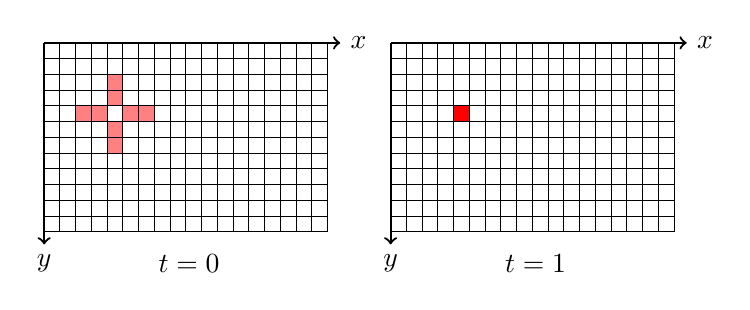
\begin{tikzpicture}[scale=.8]
\fill[red!50!white] (0.5,2) rectangle (1,1.75);
\fill[red!50!white] (1.25,2) rectangle (1.75,1.75);
\fill[red!50!white] (1,2.5) rectangle (1.25,2);
\fill[red!50!white] (1,1.25) rectangle (1.25,1.75);
\draw[xstep=.25cm,ystep=.25cm] (0,0) grid (4.5,3);
\draw[thick,->] (0,3) -- (4.7,3) node[right]{$x$};
\draw[thick,->] (0,3) -- (0,-.2) node[below]{$y$};
\draw (2.3,-.5) node {$t=0$};

\fill[red] (6.5,2) rectangle (6.75,1.75);
\draw[xstep=.25cm,ystep=.25cm] (5.5,0) grid (10,3);
\draw[thick,->] (5.5,3) -- (10.2,3) node[right]{$x$};
\draw[thick,->] (5.5,3) -- (5.5,-.2) node[below]{$y$};
\draw (7.8,-.5) node {$t=1$};
\end{tikzpicture}
\end{center}

\begin{itemize}
	\item Determine the value of a point
	\item Need values of neighbours in \emph{previous} time iteration
	\item \emph{Space-order} gives radius (\(\delta\))
\end{itemize}
\end{frame}

\begin{frame}
\frametitle{Non-problem: iteration space \(<\) cache size}

\begin{center}
	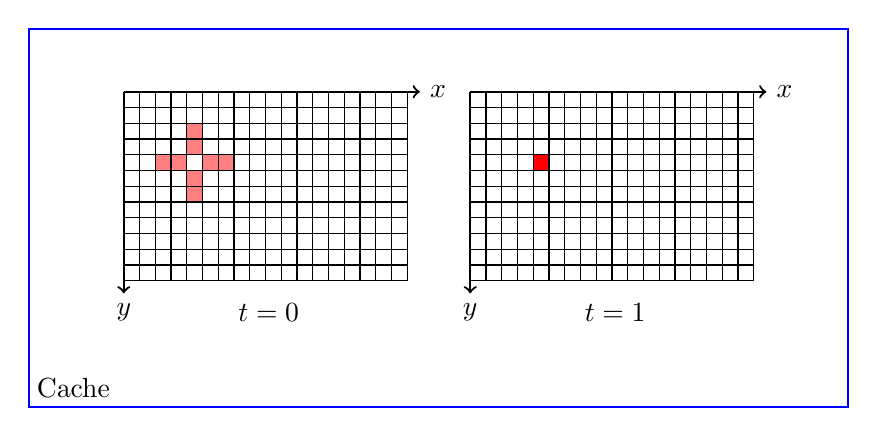
\begin{tikzpicture}[scale=.8]
	\draw[blue,thick] (-1.5,4) rectangle (11.5,-2);
	\draw (-.8,-1.7) node {Cache};

	\fill[red!50!white] (0.5,2) rectangle (1,1.75);
	\fill[red!50!white] (1.25,2) rectangle (1.75,1.75);
	\fill[red!50!white] (1,2.5) rectangle (1.25,2);
	\fill[red!50!white] (1,1.25) rectangle (1.25,1.75);
	\draw[xstep=.25cm,ystep=.25cm] (0,0) grid (4.5,3);
	\draw[thick,->] (0,3) -- (4.7,3) node[right]{$x$};
	\draw[thick,->] (0,3) -- (0,-.2) node[below]{$y$};
	\draw (2.3,-.5) node {$t=0$};

	\fill[red] (6.5,2) rectangle (6.75,1.75);
	\draw[xstep=.25cm,ystep=.25cm] (5.5,0) grid (10,3);
	\draw[thick,->] (5.5,3) -- (10.2,3) node[right]{$x$};
	\draw[thick,->] (5.5,3) -- (5.5,-.2) node[below]{$y$};
	\draw (7.8,-.5) node {$t=1$};
	\end{tikzpicture}
\end{center}

\begin{itemize}
	\item If iteration space \(<\) cache, no need to reload data
	\item Everything loaded once \Smiley
\end{itemize}
\end{frame}



\begin{frame}
\frametitle{Problem: iteration space \(>\) cache size}

\begin{center}
	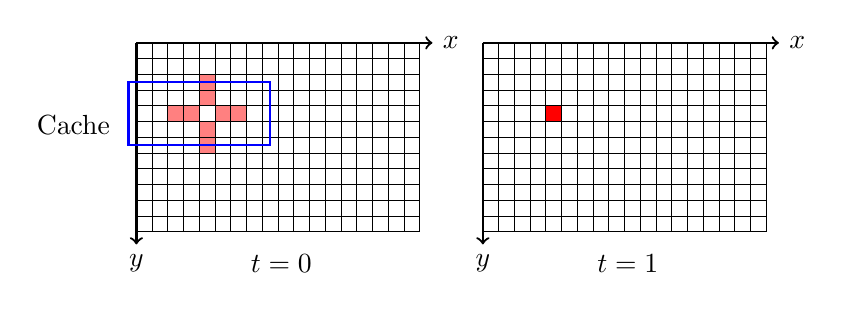
\begin{tikzpicture}[scale=.8]
	\fill[red!50!white] (0.5,2) rectangle (1,1.75);
	\fill[red!50!white] (1.25,2) rectangle (1.75,1.75);
	\fill[red!50!white] (1,2.5) rectangle (1.25,2);
	\fill[red!50!white] (1,1.25) rectangle (1.25,1.75);
	\draw[xstep=.25cm,ystep=.25cm] (0,0) grid (4.5,3);
	\draw[thick,->] (0,3) -- (4.7,3) node[right]{$x$};
	\draw[thick,->] (0,3) -- (0,-.2) node[below]{$y$};
	\draw (2.3,-.5) node {$t=0$};

	\fill[red] (6.5,2) rectangle (6.75,1.75);
	\draw[xstep=.25cm,ystep=.25cm] (5.5,0) grid (10,3);
	\draw[thick,->] (5.5,3) -- (10.2,3) node[right]{$x$};
	\draw[thick,->] (5.5,3) -- (5.5,-.2) node[below]{$y$};
	\draw (7.8,-.5) node {$t=1$};

	\draw[blue,thick] (-.125,2.375) rectangle (2.125,1.375);
	\draw (-1,1.7) node {Cache};
	\end{tikzpicture}
\end{center}

\begin{itemize}
	\item Load neighbours (t=0) into cache, some reuse in t=1 row
	\item Evicted by the time we reach end of row
	\item But we need to reload the rows again
	\item Everything loaded 3 times \Sadey
\end{itemize}
\end{frame}



\begin{frame}
\frametitle{Solution: pretend iteration space \(<\) cache size}

\begin{center}
	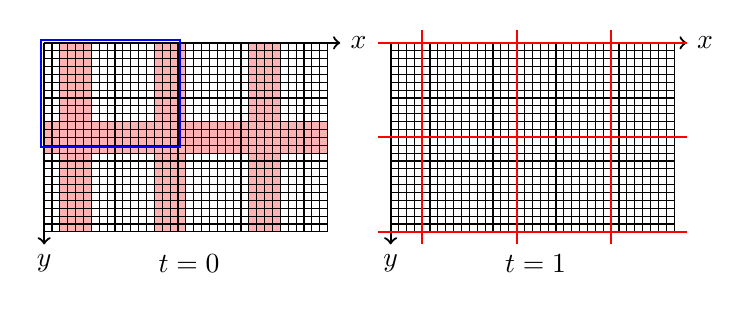
\begin{tikzpicture}[scale=.8]
	\fill[red!30!white] (0,1.25) rectangle (4.5,1.75);
	\fill[red!30!white] (0.25,0) rectangle (.75,3);
	\fill[red!30!white] (1.75,0) rectangle (2.25,3);
	\fill[red!30!white] (3.25,0) rectangle (3.75,3);
	\draw[xstep=.125cm,ystep=.125cm,thin] (0,0) grid (4.5,3);
	\draw[thick,->] (0,3) -- (4.7,3) node[right]{$x$};
	\draw[thick,->] (0,3) -- (0,-.2) node[below]{$y$};
	\draw (2.3,-.5) node {$t=0$};

	\draw[xstep=.125cm,ystep=.125cm,thin] (5.5,0) grid (10,3);
	\draw[thick,->] (5.5,3) -- (10.2,3) node[right]{$x$};
	\draw[thick,->] (5.5,3) -- (5.5,-.2) node[below]{$y$};
	\draw (7.8,-.5) node {$t=1$};
	\draw[red,thick,xstep=1.5cm,ystep=1.5cm] (5.3,-.2) grid (10.2,3.2);

	\draw[blue,thick] (-.05,3.05) rectangle (2.15,1.35);
	\end{tikzpicture}
\end{center}

\begin{itemize}
	\item Insight: x,y can be calculated in any order (parallel!)
	\item Partition into \emph{tiles}
	\item Only tile boundaries loaded twice
	\item `Exploiting data locality'
\end{itemize}
\end{frame}



\begin{frame}
\frametitle{When tiling (doesn't) work}

\begin{itemize}
	\item If compute bounded, optimising cache doesn't help much...
	\item If memory bounded, less data transfer \(\rightarrow\) faster
	\item Devito: we can make compute bounded stencils more memory bounded (cite)
	\item We needed to be able to permute x and y
	\item But can only take 1 time step at a time
\end{itemize}
\end{frame}



\begin{frame}
\frametitle{Can't interchange these loops}

\begin{center}
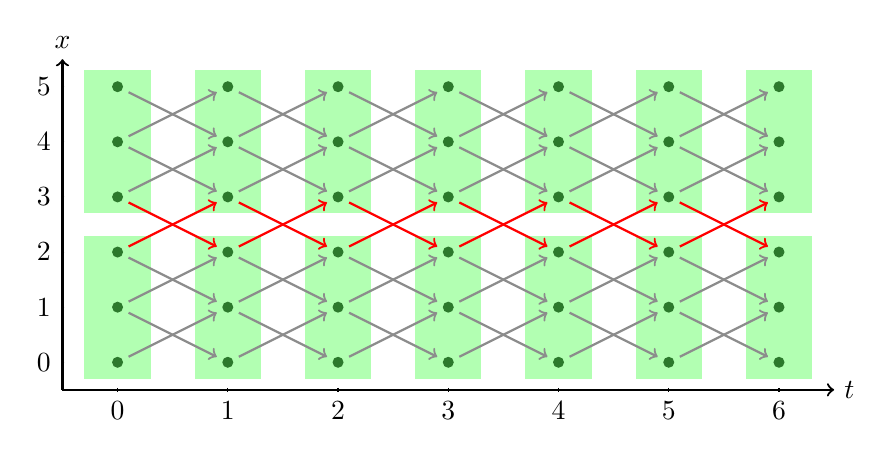
\begin{tikzpicture}[scale=0.7]
\draw[thick,->] (-1,-.5) -- (13,-.5) node[right]{$t$};
\draw[thick,->] (-1,-.5) -- (-1,5.5) node[above]{$x$};

\foreach \t in {0,1,2,3,4,5,6}
\foreach \x in {0,1,2,3,4,5}
\fill[darkgray] (\t*2,\x) circle (0.1);

\foreach \t in {0,1,2,3,4,5,6}
\foreach \x in {0,3}
\fill[green,opacity=0.3] (\t*2-.6,\x-.3) rectangle (\t*2+.6,\x+2.3);

\foreach \t in {0,1,2,3,4,5}
\foreach \x in {1,2,4,5}
\draw[thick,->,darkgray!60] (\t*2+.2,\x-.1) -- (\t*2+1.8,\x-.9);
\foreach \t in {0,1,2,3,4,5}
\foreach \x in {3}
\draw[thick,->,red] (\t*2+.2,\x-.1) -- (\t*2+1.8,\x-.9);

\foreach \t in {0,1,2,3,4,5}
\foreach \x in {0,1,3,4}
\draw[thick,->,darkgray!60] (\t*2+.2,\x+.1) -- (\t*2+1.8,\x+.9);
\foreach \t in {0,1,2,3,4,5}
\foreach \x in {2}
\draw[thick,->,red] (\t*2+.2,\x+.1) -- (\t*2+1.8,\x+.9);

\foreach \t in {0,1,2,3,4,5,6}
\draw (\t*2,1pt-.5cm) -- (\t*2,-1pt-.5cm) node[anchor=north] {$\t$};
\foreach \x in {0,1,2,3,4,5}
\draw (1pt-1cm,\x) -- (-1pt-1cm,\x) node[anchor=east] {$\x$};
\end{tikzpicture}
\end{center}

\begin{itemize}
	\item Dependencies between rows flow two ways
\end{itemize}
\end{frame}



\begin{frame}
\frametitle{Idea: skewed tiling for interchange}

\begin{center}
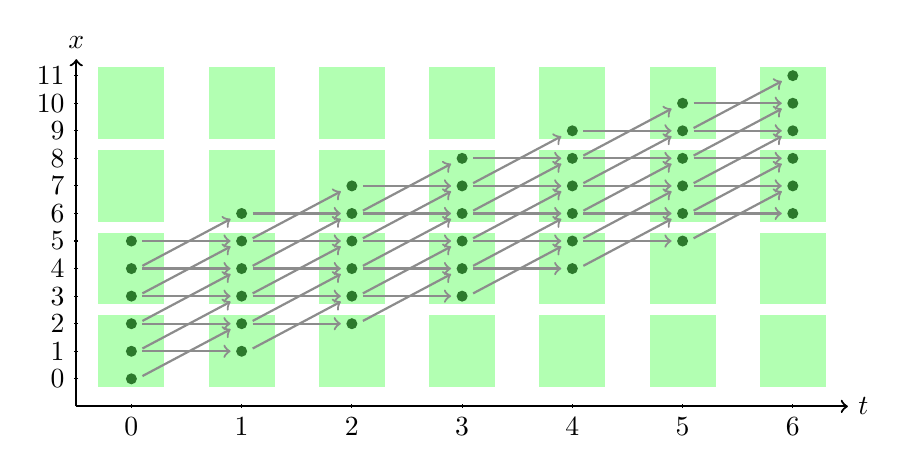
\begin{tikzpicture}[scale=0.7]
\draw[thick,->] (-1,-.5) -- (13,-.5) node[right]{$t$};
\draw[thick,->] (-1,-.5) -- (-1,5.8) node[above]{$x$};

\foreach \t in {0,1,2,3,4,5,6}
\foreach \x in {0,1,2,3,4,5}
\fill[darkgray] (\t*2,\x/2+\t/2) circle (0.1);

\foreach \t in {0,1,2,3,4,5,6}
\foreach \x in {0,3,6,9}
\fill[green,opacity=0.3] (\t*2-.6,\x/2-.15) rectangle (\t*2+.6,\x/2+1.15);

\foreach \t in {0,1,2,3,4,5}
\foreach \x in {1,2,3,4,5}
\draw[thick,->,darkgray!60] (\t*2+.2,\x/2+\t/2) -- (\t*2+1.8,\x/2+\t/2);

\foreach \t in {0,1,2,3,4,5}
\foreach \x in {0,1,2,3,4}
\draw[thick,->,darkgray!60] (\t*2+.2,\x/2+\t/2+.05) -- (\t*2+1.8,\x/2+\t/2+.9);

\foreach \t in {0,1,2,3,4,5,6}
\draw (\t*2,1pt-.5cm) -- (\t*2,-1pt-.5cm) node[anchor=north] {$\t$};
\foreach \x in {0,1,2,3,4,5,6,7,8,9,10,11}
\draw (1pt-1cm,\x/2) -- (-1pt-1cm,\x/2) node[anchor=east] {$\x$};
\end{tikzpicture}
\end{center}

\begin{itemize}
	\item Less transfer: if a tile fits in cache, can calculate subsequent tiles in that row from cache \Smiley
\end{itemize}
\end{frame}



\begin{frame}
\frametitle{Time-tiling: some important details}

\begin{itemize}
	\item Minimum skew: the distance of the spatial dependence
	\item Out of bounds accesses
	\item Only works for perfect loop nests (show imperfect)
	\item Parallelism?? (will discuss, ?? for rhetorical effect)
\end{itemize}
\end{frame}



\section{Implementing time-tiling in Devito}

\begin{frame}
\frametitle{Implemented time-tiling transformation}

\begin{itemize}
	\item Bounding using min/max functions
	\item Reasoning about tile boundaries is tricky! (example)
	\item Only works on perfect loop nests \Sadey
	\item Test cases
	\item Numerically exact (on floats!) in evaluation
\end{itemize}
\end{frame}



\begin{frame}
\frametitle{Auto-tuning tile sizes}

\begin{itemize}
	\item Parametrisation: can change tile sizes at runtime for tuning
	\item Extended auto-tuner
	\item Test only tile sizes, not skew factor
\end{itemize}
\end{frame}



\begin{frame}
\frametitle{TODOs}

\begin{itemize}
	\item Tile imperfectly-nested loops (sources and receivers) -- hard
	\item Advanced stencil optimisations -- not too hard, but maybe uses associativity of floats \Sadey
	\item Skew factor detection
	\item Time dimension buffering
\end{itemize}
\end{frame}



\section{Evaluation methodology}

\begin{frame}
\frametitle{Objectives of evaluation}

\begin{itemize}
	\item Measure speedup
	\item Find conditions for speedup
	\item Determine which stencils benefit the most
	\item Error checking
\end{itemize}
\end{frame}



\begin{frame}
\frametitle{Arithmetic intensity: how much does a stencil use data?}

\begin{itemize}
	\item Floating point operations per byte transferred from memory
	\item More operations \(\rightarrow\) more computational resources needed
	\item Fewer operations \(\rightarrow\) more memory bandwidth needed
	\item Time-tiling: most effective with low arithmetic intensity
	\item (Discuss estimator?)
\end{itemize}
\end{frame}



\begin{frame}
\frametitle{Time-tiling increases arithmetic intensity}

\begin{itemize}
	\item Time-tiling: improve cache reuse
	\item More reuse \(\rightarrow\) more operations per byte
	\item Effectively increases the arithmetic intensity of a stencil
\end{itemize}
\end{frame}



\begin{frame}
\frametitle{Testing framework}

\begin{itemize}
	\item CSG Intel Xeon E5-2470; 8 cores, 16 threads, 20MB L3 cache
	\item 64GB DRAM
	\item OpenMP: parallelism, use all threads, prevent migration
	\item Intel C Compiler, all optimisations enabled
	\item Devito auto-tuner to ensure best runtime
	\item Always verify functional correctness
	\item Minimum runtime reported
\end{itemize}
\end{frame}



\begin{frame}
\frametitle{Performance bounds}

\begin{itemize}
	\item Limits that cannot be exceeded
	\item 294.4 = something
	\item LINPACK: 262 GFlops (cite...)
	\item STREAM: 17.3 GB/s
\end{itemize}
\end{frame}



\begin{frame}
\frametitle{Roofline (cite)}

\begin{center}
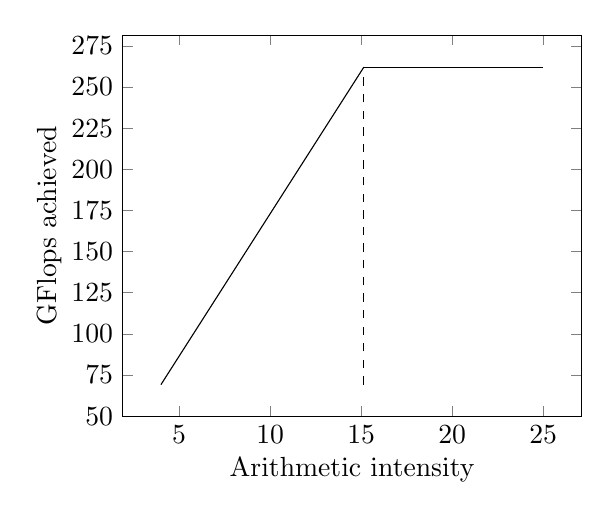
\begin{tikzpicture}[scale=0.85]
\begin{axis}[
legend style={at={(0.95,0.05)},anchor=south east},
xlabel={Arithmetic intensity},
ylabel={GFlops achieved},
ytick distance=25,
]
% roofline
\addplot [domain=4:15.15,name path=A] {17.3*x};
\addplot [domain=15.15:25] {262.01};
% boundary
\path[name path=X] (4, 0) -- (200, 0);
\addplot[gray, pattern=north west lines] fill between[of=A and X, soft clip={domain=4:15.15}];
\addplot +[mark=none,dashed] coordinates {(15.15, 69.2) (15.15, 259.5)};
\end{axis}
\end{tikzpicture}
\end{center}

\begin{itemize}
	\item Memory bounded (shaded), then CPU bounded
	\item Can't exceed roofline!
\end{itemize}
\end{frame}



\begin{frame}
\frametitle{Verification}

\begin{itemize}
	\item All results numerically exact \Smiley
	\item They aren't all (or even mostly) zeroes
	\item They aren't infinity or NaN
	\item Error bound: zero
\end{itemize}
\end{frame}



\section{Results}

\begin{frame}
\frametitle{Laplace operator}

\begin{itemize}
	\item 4 stencils from the Laplace operator
	\item Generated by Devito, varying space orders
	\item Experimented on 2 grids, but only presenting 1 as results are similar
\end{itemize}
\end{frame}



\begin{frame}
\frametitle{Laplace: runtime against space order}

\begin{center}
\begin{tikzpicture}
\begin{axis}[
width=0.7\textwidth,
legend style={at={(0.05,0.95)},anchor=north west},
xlabel={Space order},
ylabel={Runtime(s)},
ytick distance=2,
]
\addplot table [x=sp,y=run,col sep=comma] {../data/laplace-nt600.csv};
\addplot table [x=sp,y=run,col sep=comma] {../data/laplace-sp600.csv};
\addplot table [x=sp,y=run,col sep=comma] {../data/laplace-tm600.csv};
\legend{Non-tiled,Space-tiling,Time-tiling}
\end{axis}
\end{tikzpicture}
\end{center}
\begin{itemize}
	\item 25\% decrease to 1\% decrease with higher arith. intensity
\end{itemize}
\end{frame}



\begin{frame}
\frametitle{Laplace: roofline}

\begin{itemize}
	\item (Reserved a slide)
\end{itemize}
\end{frame}



\begin{frame}
\frametitle{Acoustic wave equation operator}

\begin{itemize}
	\item 5 stencils from AWE operator
	\item Generated by Devito, varying space orders
	\item Experimented on a \(512^3\) + time grid
	\item `More realistic': AWE is very important in Devito's target domain, seismic imaging
	\item Lower arithmetic intensity
\end{itemize}
\end{frame}



\begin{frame}
\frametitle{AWE: runtime against space order}

\begin{center}
\begin{tikzpicture}
\begin{axis}[
width=0.7\textwidth,
legend style={at={(0.05,0.95)},anchor=north west},
xlabel={Space order},
ylabel={Runtime(s)},
ytick distance=2,
]
\addplot table [x=sp,y=run,col sep=comma] {../data/awe-nt512.csv};
\addplot table [x=sp,y=run,col sep=comma] {../data/awe-sp512.csv};
\addplot table [x=sp,y=run,col sep=comma] {../data/awe-tm512.csv};
\legend{Non-tiled,Space-tiling,Time-tiling}
\end{axis}
\end{tikzpicture}
\end{center}
\begin{itemize}
\item 45\% to 20\% decrease!
\end{itemize}
\end{frame}



\begin{frame}
\frametitle{AWE: roofline}

\begin{itemize}
\item (Reserved a slide)
\end{itemize}
\end{frame}



\begin{frame}
\frametitle{Effect of time tile size}

\begin{itemize}
	\item Low space order: big time tiles
	\item High space order: not much benefit after tile sizes 4, 8
	\item Non-trivial tile boundary overlap and finite cache \(\rightarrow\) arithmetic intensity overestimated
\end{itemize}
\end{frame}



\begin{frame}
\frametitle{Effect of skewing factor}

\begin{itemize}
	\item No change to arith. intensity
	\item (I didn't include the tables: should I?)
	\item Smallest valid skewing factor is fastest: even 3, 6
	\item Possibly because we need to load the neighbours anyway, so misalignment not an issue
\end{itemize}
\end{frame}



\begin{frame}
\frametitle{Further evaluation work}

\begin{itemize}
	\item Implementation -- only perfect loops
	\item Test more architectures
	\item Analyse memory to check cache misses, new bottlenecks
\end{itemize}
\end{frame}



\section{Conclusion}

\begin{frame}
\frametitle{}

\begin{itemize}
	\item Contributions?
	\item What else?
	\item 
	\item 
\end{itemize}
\end{frame}



\begin{frame}
\frametitle{Things to ask Paul}

\begin{itemize}
	\item Related work in presentation?
	\item Talk about the individual transformation? (e.g. code for skewing \Sadey)
	\item 
	\item 
\end{itemize}
\end{frame}



%\begin{frame}
%\frametitle{}
%
%\begin{itemize}
%	\item 
%	\item 
%	\item 
%	\item 
%\end{itemize}
%\end{frame}


\end{document}